% Results report: heights film validation study (confirmatory sample).
% Every number comes from manuscript/generated/ (written by analysis/05_report_numbers.py); none is typed by hand.
% Build:  cd manuscript && latexmk -pdf results.tex
\documentclass[man,floatsintext,12pt,donotrepeattitle]{apa7}

\usepackage[american]{babel}
\usepackage[T1]{fontenc}
\usepackage{newtxtext,newtxmath} % Times-style; heavier strokes than Latin Modern, easier to read on screens
\usepackage{booktabs}
\usepackage{array}
\usepackage{graphicx}
\usepackage{amsmath}
\usepackage{csquotes}
\graphicspath{{../results/confirmatory/figures/}}

% Written by analysis/05_report_numbers.py - do not edit by hand.
\newcommand{\val}[1]{\ifcsname val:#1\endcsname\csname val:#1\endcsname\else\errmessage{Unknown value #1}\fi}
\expandafter\def\csname val:n_completed\endcsname{130}
\expandafter\def\csname val:n_excluded\endcsname{6}
\expandafter\def\csname val:n_primary\endcsname{124}
\expandafter\def\csname val:n_excl_disrupted\endcsname{3}
\expandafter\def\csname val:n_excl_freetext\endcsname{2}
\expandafter\def\csname val:n_excl_erratic\endcsname{1}
\expandafter\def\csname val:n_cohort_two\endcsname{19}
\expandafter\def\csname val:n_cohort_three\endcsname{20}
\expandafter\def\csname val:n_cohort_four\endcsname{85}
\expandafter\def\csname val:n_age\endcsname{121}
\expandafter\def\csname val:age_mean\endcsname{34.2}
\expandafter\def\csname val:age_sd\endcsname{12.0}
\expandafter\def\csname val:age_min\endcsname{18}
\expandafter\def\csname val:age_max\endcsname{76}
\expandafter\def\csname val:n_female\endcsname{59}
\expandafter\def\csname val:n_male\endcsname{62}
\expandafter\def\csname val:n_sex_missing\endcsname{3}
\expandafter\def\csname val:n_mouse\endcsname{80}
\expandafter\def\csname val:n_trackpad\endcsname{43}
\expandafter\def\csname val:n_stricter\endcsname{96}
\expandafter\def\csname val:n_sparse\endcsname{24}
\expandafter\def\csname val:n_one_check\endcsname{5}
\expandafter\def\csname val:n_not_attentive\endcsname{3}
\expandafter\def\csname val:n_without_rejected\endcsname{120}
\expandafter\def\csname val:n_rejection_set\endcsname{4}
\expandafter\def\csname val:n_exploratory_completed\endcsname{23}
\expandafter\def\csname val:n_exploratory\endcsname{21}
\expandafter\def\csname val:height_fear_mean\endcsname{3.77}
\expandafter\def\csname val:height_fear_sd\endcsname{1.73}
\expandafter\def\csname val:height_fear_median\endcsname{4}
\expandafter\def\csname val:sticsa_pre_mean\endcsname{13.76}
\expandafter\def\csname val:sticsa_pre_sd\endcsname{3.56}
\expandafter\def\csname val:sticsa_pre_median\endcsname{13}
\expandafter\def\csname val:sticsa_post_mean\endcsname{20.55}
\expandafter\def\csname val:sticsa_post_sd\endcsname{7.29}
\expandafter\def\csname val:sticsa_post_median\endcsname{18}
\expandafter\def\csname val:sticsa_change_mean\endcsname{6.79}
\expandafter\def\csname val:sticsa_change_sd\endcsname{6.60}
\expandafter\def\csname val:sticsa_change_median\endcsname{5}
\expandafter\def\csname val:anxiety_overall_mean\endcsname{5.18}
\expandafter\def\csname val:anxiety_overall_sd\endcsname{1.33}
\expandafter\def\csname val:anxiety_overall_median\endcsname{5}
\expandafter\def\csname val:concern_safety_mean\endcsname{6.13}
\expandafter\def\csname val:concern_safety_sd\endcsname{1.30}
\expandafter\def\csname val:concern_safety_median\endcsname{7}
\expandafter\def\csname val:body_intensity_mean\endcsname{4.64}
\expandafter\def\csname val:body_intensity_sd\endcsname{1.60}
\expandafter\def\csname val:body_intensity_median\endcsname{5}
\expandafter\def\csname val:arousal_baseline_mean\endcsname{43.13}
\expandafter\def\csname val:arousal_baseline_sd\endcsname{15.80}
\expandafter\def\csname val:arousal_baseline_median\endcsname{43.8}
\expandafter\def\csname val:arousal_rise_mean\endcsname{67.14}
\expandafter\def\csname val:arousal_rise_sd\endcsname{14.79}
\expandafter\def\csname val:arousal_rise_median\endcsname{68.9}
\expandafter\def\csname val:arousal_plateau_mean\endcsname{80.91}
\expandafter\def\csname val:arousal_plateau_sd\endcsname{15.01}
\expandafter\def\csname val:arousal_plateau_median\endcsname{83.1}
\expandafter\def\csname val:arousal_return_mean\endcsname{53.89}
\expandafter\def\csname val:arousal_return_sd\endcsname{19.42}
\expandafter\def\csname val:arousal_return_median\endcsname{54.8}
\expandafter\def\csname val:arousal_whole_film_mean\endcsname{61.23}
\expandafter\def\csname val:arousal_whole_film_sd\endcsname{10.99}
\expandafter\def\csname val:arousal_whole_film_median\endcsname{60.6}
\expandafter\def\csname val:valence_baseline_mean\endcsname{50.58}
\expandafter\def\csname val:valence_baseline_sd\endcsname{14.55}
\expandafter\def\csname val:valence_baseline_median\endcsname{52.0}
\expandafter\def\csname val:valence_rise_mean\endcsname{39.58}
\expandafter\def\csname val:valence_rise_sd\endcsname{19.06}
\expandafter\def\csname val:valence_rise_median\endcsname{38.5}
\expandafter\def\csname val:valence_plateau_mean\endcsname{29.13}
\expandafter\def\csname val:valence_plateau_sd\endcsname{23.10}
\expandafter\def\csname val:valence_plateau_median\endcsname{23.9}
\expandafter\def\csname val:valence_return_mean\endcsname{50.84}
\expandafter\def\csname val:valence_return_sd\endcsname{20.44}
\expandafter\def\csname val:valence_return_median\endcsname{51.7}
\expandafter\def\csname val:valence_whole_film_mean\endcsname{41.89}
\expandafter\def\csname val:valence_whole_film_sd\endcsname{14.67}
\expandafter\def\csname val:valence_whole_film_median\endcsname{41.9}
\expandafter\def\csname val:H1:report\endcsname{$t$(123) = 11.46, $p$ < .001, $d_z$ = 1.03, 95\% CI [0.81, 1.25]}
\expandafter\def\csname val:H1:effect\endcsname{$d_z$ = 1.03 [0.81, 1.25]}
\expandafter\def\csname val:H1:est\endcsname{1.03}
\expandafter\def\csname val:H1:diff\endcsname{6.79}
\expandafter\def\csname val:H1:diffabs\endcsname{6.79}
\expandafter\def\csname val:H2a:report\endcsname{$t$(123) = 14.67, $p_\mathrm{Holm}$ < .001, $d_z$ = 1.32, 95\% CI [1.07, 1.56]}
\expandafter\def\csname val:H2a:effect\endcsname{$d_z$ = 1.32 [1.07, 1.56]}
\expandafter\def\csname val:H2a:est\endcsname{1.32}
\expandafter\def\csname val:H2a:diff\endcsname{24.01}
\expandafter\def\csname val:H2a:diffabs\endcsname{24.01}
\expandafter\def\csname val:H2b:report\endcsname{$t$(123) = 19.77, $p_\mathrm{Holm}$ < .001, $d_z$ = 1.78, 95\% CI [1.49, 2.06]}
\expandafter\def\csname val:H2b:effect\endcsname{$d_z$ = 1.78 [1.49, 2.06]}
\expandafter\def\csname val:H2b:est\endcsname{1.78}
\expandafter\def\csname val:H2b:diff\endcsname{37.78}
\expandafter\def\csname val:H2b:diffabs\endcsname{37.78}
\expandafter\def\csname val:H2c:report\endcsname{$t$(123) = $-$14.70, $p_\mathrm{Holm}$ < .001, $d_z$ = $-$1.32, 95\% CI [$-$1.56, $-$1.08]}
\expandafter\def\csname val:H2c:effect\endcsname{$d_z$ = $-$1.32 [$-$1.56, $-$1.08]}
\expandafter\def\csname val:H2c:est\endcsname{$-$1.32}
\expandafter\def\csname val:H2c:diff\endcsname{$-$27.02}
\expandafter\def\csname val:H2c:diffabs\endcsname{27.02}
\expandafter\def\csname val:H2d:report\endcsname{$t$(123) = $-$9.85, $p_\mathrm{Holm}$ < .001, $d_z$ = $-$0.88, 95\% CI [$-$1.09, $-$0.68]}
\expandafter\def\csname val:H2d:effect\endcsname{$d_z$ = $-$0.88 [$-$1.09, $-$0.68]}
\expandafter\def\csname val:H2d:est\endcsname{$-$0.88}
\expandafter\def\csname val:H2d:diff\endcsname{$-$21.44}
\expandafter\def\csname val:H2d:diffabs\endcsname{21.44}
\expandafter\def\csname val:H3arousal:report\endcsname{$r$ = .993, 95\% CI [.990, .996]}
\expandafter\def\csname val:H3arousal:effect\endcsname{$r$ = .993 [.990, .996]}
\expandafter\def\csname val:H3arousal:est\endcsname{.99}
\expandafter\def\csname val:H3valence:report\endcsname{$r$ = .937, 95\% CI [.893, .966]}
\expandafter\def\csname val:H3valence:effect\endcsname{$r$ = .937 [.893, .966]}
\expandafter\def\csname val:H3valence:est\endcsname{.94}
\expandafter\def\csname val:H4a:report\endcsname{$\rho$ = .08, 95\% CI [$-$.09, .26], $p$ = .355, $p_\mathrm{Holm}$ = .355}
\expandafter\def\csname val:H4a:effect\endcsname{$\rho$ = .08 [$-$.09, .26]}
\expandafter\def\csname val:H4a:est\endcsname{.08}
\expandafter\def\csname val:H4b:report\endcsname{$\rho$ = $-$.32, 95\% CI [$-$.46, $-$.16], $p$ < .001, $p_\mathrm{Holm}$ = .001}
\expandafter\def\csname val:H4b:effect\endcsname{$\rho$ = $-$.32 [$-$.46, $-$.16]}
\expandafter\def\csname val:H4b:est\endcsname{$-$.32}
\expandafter\def\csname val:H4c:report\endcsname{$\rho$ = .18, 95\% CI [.00, .35], $p$ = .049, $p_\mathrm{Holm}$ = .098}
\expandafter\def\csname val:H4c:effect\endcsname{$\rho$ = .18 [.00, .35]}
\expandafter\def\csname val:H4c:est\endcsname{.18}
\expandafter\def\csname val:H5a:report\endcsname{$\rho$ = .24, 95\% CI [.05, .41], $p$ = .008, $p_\mathrm{Holm}$ = .008}
\expandafter\def\csname val:H5a:effect\endcsname{$\rho$ = .24 [.05, .41]}
\expandafter\def\csname val:H5a:est\endcsname{.24}
\expandafter\def\csname val:H5b:report\endcsname{$\rho$ = $-$.38, 95\% CI [$-$.51, $-$.23], $p$ < .001, $p_\mathrm{Holm}$ < .001}
\expandafter\def\csname val:H5b:effect\endcsname{$\rho$ = $-$.38 [$-$.51, $-$.23]}
\expandafter\def\csname val:H5b:est\endcsname{$-$.38}
\expandafter\def\csname val:H6a:report\endcsname{$\rho$ = .56, 95\% CI [.44, .67], $p$ < .001, $p_\mathrm{Holm}$ < .001}
\expandafter\def\csname val:H6a:effect\endcsname{$\rho$ = .56 [.44, .67]}
\expandafter\def\csname val:H6a:est\endcsname{.56}
\expandafter\def\csname val:H6b:report\endcsname{$\rho$ = .34, 95\% CI [.15, .50], $p$ < .001, $p_\mathrm{Holm}$ < .001}
\expandafter\def\csname val:H6b:effect\endcsname{$\rho$ = .34 [.15, .50]}
\expandafter\def\csname val:H6b:est\endcsname{.34}
\expandafter\def\csname val:H2:absrange\endcsname{0.88--1.78}
\expandafter\def\csname val:H1:wilcoxon\endcsname{$T$ = 197, $p$ < .001}
\expandafter\def\csname val:n_floor_pre\endcsname{45}
\expandafter\def\csname val:pct_floor_pre\endcsname{36}
\expandafter\def\csname val:n_increase\endcsname{109}
\expandafter\def\csname val:n_nochange\endcsname{7}
\expandafter\def\csname val:n_decrease\endcsname{8}
\expandafter\def\csname val:n_fear_top\endcsname{20}
\expandafter\def\csname val:n_fear_seven\endcsname{2}
\expandafter\def\csname val:rel:arousal\endcsname{.992}
\expandafter\def\csname val:rel:valence\endcsname{.979}
\expandafter\def\csname val:edge1:est\endcsname{262}
\expandafter\def\csname val:edge1:reg\endcsname{262}
\expandafter\def\csname val:edge1:ci\endcsname{[133, 271]}
\expandafter\def\csname val:edge2:est\endcsname{467}
\expandafter\def\csname val:edge2:reg\endcsname{470}
\expandafter\def\csname val:edge2:ci\endcsname{[317, 475]}
\expandafter\def\csname val:edge3:est\endcsname{660}
\expandafter\def\csname val:edge3:reg\endcsname{692}
\expandafter\def\csname val:edge3:ci\endcsname{[631, 690]}
\expandafter\def\csname val:confirmatory_commit\endcsname{63d042d}
\expandafter\def\csname val:seed\endcsname{20261004}
\expandafter\def\csname val:python_version\endcsname{3.13.7}
\expandafter\def\csname val:version:numpy\endcsname{2.5.3}
\expandafter\def\csname val:version:pandas\endcsname{3.0.6}
\expandafter\def\csname val:version:scipy\endcsname{1.18.1}
\expandafter\def\csname val:version:matplotlib\endcsname{3.11.2}
\expandafter\def\csname val:version:statsmodels\endcsname{0.15.0}
\expandafter\def\csname val:n_demo\endcsname{121}
\expandafter\def\csname val:n_demo_female\endcsname{59}
\expandafter\def\csname val:n_demo_male\endcsname{62}
\expandafter\def\csname val:change_female_mean\endcsname{7.17}
\expandafter\def\csname val:change_male_mean\endcsname{6.44}
\expandafter\def\csname val:agesex:change_sex\endcsname{0.66 [$-$1.77, 3.08], $p$ = .593}
\expandafter\def\csname val:agesex:change_age\endcsname{0.24 [$-$0.78, 1.25], $p$ = .645}
\expandafter\def\csname val:agesex:arousal:sex_x_segment\endcsname{$\chi^2$(3) = 0.28, $p$ = .964}
\expandafter\def\csname val:agesex:arousal:sex_x_segment:check\endcsname{$F$(3, 120) = 0.08, $p$ = .969}
\expandafter\def\csname val:agesex:arousal:age_x_segment\endcsname{$\chi^2$(3) = 4.92, $p$ = .178}
\expandafter\def\csname val:agesex:arousal:age_x_segment:check\endcsname{$F$(3, 120) = 2.13, $p$ = .100}
\expandafter\def\csname val:agesex:arousal:female_minus_male\endcsname{$-$0.50 [$-$4.47, 3.47], $p$ = .806}
\expandafter\def\csname val:agesex:arousal:per_10_years\endcsname{$-$1.26 [$-$2.88, 0.37], $p$ = .129}
\expandafter\def\csname val:agesex:valence:sex_x_segment\endcsname{$\chi^2$(3) = 0.72, $p$ = .869}
\expandafter\def\csname val:agesex:valence:sex_x_segment:check\endcsname{$F$(3, 120) = 0.43, $p$ = .734}
\expandafter\def\csname val:agesex:valence:age_x_segment\endcsname{$\chi^2$(3) = 1.84, $p$ = .607}
\expandafter\def\csname val:agesex:valence:age_x_segment:check\endcsname{$F$(3, 120) = 0.50, $p$ = .682}
\expandafter\def\csname val:agesex:valence:female_minus_male\endcsname{$-$4.46 [$-$9.91, 0.99], $p$ = .108}
\expandafter\def\csname val:agesex:valence:per_10_years\endcsname{$-$0.74 [$-$2.96, 1.47], $p$ = .511}
\expandafter\def\csname val:agesex:valence_rise_diff\endcsname{$-$6.43 points [$-$13.19, 0.34], $p$ = .062}
\expandafter\def\csname val:items:dz_min\endcsname{0.52}
\expandafter\def\csname val:items:dz_max\endcsname{1.17}
\expandafter\def\csname val:items:pholm_max\endcsname{< .001}
\expandafter\def\csname val:items:rank1:label\endcsname{heart beats fast}
\expandafter\def\csname val:items:rank1:dz\endcsname{1.17}
\expandafter\def\csname val:items:rank2:label\endcsname{trembly, shaky}
\expandafter\def\csname val:items:rank2:dz\endcsname{0.80}
\expandafter\def\csname val:items:rank3:label\endcsname{breathing fast, shallow}
\expandafter\def\csname val:items:rank3:dz\endcsname{0.77}
\expandafter\def\csname val:items:rank4:label\endcsname{muscles tense}
\expandafter\def\csname val:items:rank4:dz\endcsname{0.72}
\expandafter\def\csname val:items:rank5:label\endcsname{dizzy}
\expandafter\def\csname val:items:rank5:dz\endcsname{0.71}
\expandafter\def\csname val:items:rank6:label\endcsname{face hot}
\expandafter\def\csname val:items:rank6:dz\endcsname{0.66}
\expandafter\def\csname val:items:rank7:label\endcsname{butterflies in stomach}
\expandafter\def\csname val:items:rank7:dz\endcsname{0.64}
\expandafter\def\csname val:items:rank8:label\endcsname{palms clammy}
\expandafter\def\csname val:items:rank8:dz\endcsname{0.60}
\expandafter\def\csname val:items:rank9:label\endcsname{throat dry}
\expandafter\def\csname val:items:rank9:dz\endcsname{0.54}
\expandafter\def\csname val:items:rank10:label\endcsname{muscles weak}
\expandafter\def\csname val:items:rank10:dz\endcsname{0.52}
\expandafter\def\csname val:items:rank11:label\endcsname{arms and legs stiff}
\expandafter\def\csname val:items:rank11:dz\endcsname{0.52}
\expandafter\def\csname val:task:valence\endcsname{20}
\expandafter\def\csname val:task:arousal\endcsname{88}


\title{Moment-to-Moment Affect During Film-Induced Somatic Anxiety}
\shorttitle{Moment-to-Moment Affect}
\author{Micah G. Allen}
\affiliation{Center of Functionally Integrative Neuroscience, Aarhus University}
\authornote{Draft Methods and Results for internal review. Preregistration: \url{https://osf.io/s2yvb}. The
confirmatory tests were run on the confirmatory sample from commit \texttt{\val{confirmatory_commit}} (random seed
\val{seed}); every number in this document is generated directly from those outputs.}

\begin{document}
\maketitle

\section{Method}

The study was preregistered on the Open Science Framework before any hypothesis test was run
(\url{https://osf.io/s2yvb}). Hypotheses, segment edges, exclusion rules, tests, correction families and inference
criteria are reported here as registered, and anything not in the registration is labelled exploratory. Decisions
taken after registration are recorded, with dates, in the project's preregistration log and summarized at the end of
the Results.

\subsection{Participants}

Participants were recruited on Prolific. Eligibility filters were fluent English, normal or corrected-to-normal
vision, an approval rate of at least 95\%, at least 20 previous submissions and a desktop computer; the study listing
and information sheet also required a physical mouse or trackpad. Recruitment ran in cohorts. Each cohort was a
separate Prolific study with a 50/50 quota on Prolific's sex screener, and participants from earlier cohorts were
blocked from later ones. Cohort 4 was a single study whose places were increased in steps of 20 about 25 minutes
apart, which limited the number of simultaneous video downloads. Participants were paid \pounds 4.80 for an estimated
30 minutes. The information sheet advised people with a strong fear of heights not to take part, and consent included
the statement \enquote{I do not expect this to be seriously distressing for me.} The study was conducted under the
Aarhus University standard waiver for non-interventional online studies.

The pilot and cohort 1 form the exploratory sample, which was used to set the segment edges, the exclusion rules and
the sample size. Cohorts 2--4 form the confirmatory sample, and all confirmatory tests use only these participants.
The registered target was 120 usable confirmatory participants, with recruitment stopping at the end of the first
cohort after which this number was reached. This sample size gives 80\% power to detect correlations of about .25
(two-sided $\alpha$~=~.05); the within-participant effects in the exploratory data were far larger.

\subsection{Stimulus}

The film shows people climbing a skyscraper from a first-person view. It lasts 13 min 28 s and was presented without
sound (H.264, 1280~$\times$~720 pixels, 25 frames per second). The whole file was downloaded before playback began;
if the download did not finish within 5 minutes, the session ended and the participant was asked to return the
study.

\subsection{Procedure}

The task ran in the browser (jsPsych 8 on JATOS). After giving consent, participants passed a device check (desktop
computer, browser window of at least 1000~$\times$~600 pixels), rated their everyday fear of heights and completed
the first attention check. The study then switched to full screen. Participants read the instructions and practised
the rating task: they tracked a moving target on the two-dimensional grid for 40~s (repeated once if the tracking
error exceeded 20 units) and then placed six example emotional states on the grid.

Participants then completed the STICSA somatic scale, watched the film while rating continuously, and completed the
STICSA somatic scale again immediately afterwards. The session ended with the post-film questions, the second
attention check, a written description of the experience of at least 100 words and an optional feedback field. If
participants switched tabs, left full screen or released the mouse pointer, the film paused until they returned.

\subsection{Measures}

\subsubsection{Continuous Valence and Arousal}

Throughout the film, participants moved a dot within a small affect grid in the corner of the video using the mouse
(pointer locked). The horizontal position coded valence (0~=~unpleasant, 50~=~neutral, 100~=~pleasant) and the
vertical position coded arousal (0~=~low, 100~=~high activation). The position was sampled at 20~Hz and time-stamped
against film playback time.

\subsubsection{Somatic Anxiety}

State somatic anxiety was measured with the somatic subscale of the State-Trait Inventory for Cognitive and Somatic
Anxiety (STICSA; state form), immediately before and immediately after the film, with the instruction
\enquote{Please indicate how you feel right now, at this moment.} The subscale has 11 items (items 1, 2, 6, 7, 8, 12,
14, 15, 18, 20 and 21), each answered from 1 (\emph{not at all}) to 4 (\emph{very much so}). The total ranges from 11
to 44 and was computed only when all items were answered; the change score is post minus pre.

\subsubsection{Single-Item Ratings}

Before the film, participants answered \enquote{In everyday life, how afraid are you of heights?} from 1 (\emph{not
at all}) to 7 (\emph{extremely}). After the film, they rated on 1--7 scales how tense or anxious they had felt overall
while watching (\enquote{Overall, how tense or anxious did you feel while watching the film?}), how concerned they
had been for the safety of the people in the film, and how strong their bodily sensations had been. They also
reported whether they had seen the film before, whether they had watched attentively and which input device they had
used.

\subsection{Data Processing}

For each participant, the 20-Hz ratings were resampled to 1~Hz of film time (808 values, 0--807~s) by linear
interpolation over the samples recorded while the film was playing. The film was divided into four segments with
edges fixed in advance: baseline (0--262~s), rise (262--470~s), plateau (470--692~s) and return (692--808~s). These
edges had been estimated in the exploratory sample by piecewise-linear segmentation of the group-mean arousal series.
A participant's segment mean is the mean of their 1-Hz series within a segment, and the whole-film mean is the mean
over all 808 values. Group-mean series are the mean across participants at each second.

\subsection{Exclusions}

Participants who completed the study were excluded if any of seven registered rules applied, all decided from
data-quality logs without reference to the hypotheses: (a) failing both attention checks; (b) script-generated input
events during the film; (c) a written description that was not typed (keystrokes fewer than 0.2 times the number of
characters, for texts of at least 200 characters); (d) erratic input (more than 10\% of mouse movements larger than
250 pixels); (e) disrupted viewing (more than 30~s of buffering or more than 60~s of interruptions during the film);
(f) ratings recorded during fewer than 95\% of the film's seconds; or (g) having seen the film before.

Two sensitivity samples were also registered, and every confirmatory test was repeated in each. The first
additionally excluded sparse raters (fewer than one rating bout per minute, where inputs more than 2~s apart start a
new bout, or a stretch of more than 180~s without input), participants who failed one of the two attention checks,
and participants who reported not watching attentively. The second additionally excluded participants whose Prolific
submissions had been rejected for their behaviour on the free-text page but who passed the registered exclusion
rules.

\subsection{Statistical Analysis}

All tests were two-sided with $\alpha$~=~.05 after Holm correction within each family of hypotheses. A directional
hypothesis was considered supported only if the effect was significant in the predicted direction.

\paragraph{H1.} STICSA somatic totals after and before the film were compared with a paired $t$ test. The effect size
is Cohen's $d_z$ (the mean of the differences divided by their standard deviation) with an exact 95\% confidence
interval from the noncentral $t$ distribution. A Wilcoxon signed-rank test was run as a robustness check.

\paragraph{H2.} Four within-participant contrasts of segment means were tested with paired $t$ tests: arousal in the
rise and on the plateau against baseline (both predicted higher), arousal in the return against the plateau
(predicted lower) and valence on the plateau against baseline (predicted lower). Effect sizes are $d_z$ with exact
95\% confidence intervals; $p$ values were Holm-corrected across the four contrasts.

\paragraph{H3.} For arousal and for valence separately, the group-mean series of the confirmatory sample was
correlated with the group-mean series of the exploratory sample (Pearson $r$ over the 808 one-second values). Because
neighbouring seconds are not independent, the 95\% confidence interval was obtained with a circular block bootstrap
over time (30-s blocks, 5,000 resamples, the same blocks drawn from both series). H3 was considered supported for a
dimension if the lower bound of this interval exceeded .50.

\paragraph{H4--H6.} The individual-difference hypotheses were tested with Spearman rank correlations across
participants, chosen because the predictors are ordinal and the outcomes bounded. H4 related everyday fear of heights
to plateau arousal (H4a, predicted positive), plateau valence (H4b, negative) and the STICSA change (H4c, positive).
H5 related the STICSA change to whole-film mean arousal (H5a, positive) and valence (H5b, negative). H6 related
post-film overall anxiety to the STICSA change (H6a, positive) and to plateau arousal (H6b, positive). Each
correlation has a percentile bootstrap 95\% confidence interval (5,000 resamples of participants), and Holm
correction was applied within H4 (three tests), H5 (two) and H6 (two). The trend lines in
Figure~\ref{fig:correlations} are least-squares fits drawn as a visual guide; they are not the tests.

\paragraph{Descriptive Analyses.} Two registered descriptive analyses accompany the tests. The reliability of the
group-mean series was estimated by splitting the participants randomly into two halves 1,000 times, correlating the
two half-sample means and applying the Spearman--Brown correction. The segment edges were re-estimated in the
confirmatory sample with the method used in the exploratory sample: an exact piecewise-linear segmentation of the
group-mean arousal series into four straight-line segments (three breakpoints, each segment at least 30~s long, found
by dynamic programming), with 95\% intervals from 1,000 bootstrap resamples of participants.

\paragraph{Exploratory Analyses.} Two analyses were not registered as tests and are reported as exploratory. The
first describes how participants occupied the affect grid in each segment. The second examines age and sex, which the
registration lists among the planned exploratory analyses. Sex was taken from participants' Prolific profiles (female
or male); Prolific withholds age and sex for rejected submissions, so these analyses include only participants with
both. The STICSA change was regressed on sex and age. For the segment means of each rating, a mixed model with a random
intercept per participant included segment (sum-coded), sex, age and the segment~$\times$~sex and segment~$\times$~age
interactions; each interaction was tested with a likelihood-ratio test (3 degrees of freedom) against the model
without it. As a check, the same model was fitted by least squares with standard errors clustered by participant and
the interactions tested with Wald $F$ tests. The age and sex analyses, including the rule that the mixed model is
the main result, were specified and tried out on the exploratory sample before they were run on the confirmatory
sample. There is no registered correction family for these
analyses, so $p$ values are uncorrected and the estimates with their confidence intervals should carry the weight.

\paragraph{Missing Data and Software.} STICSA items were required, so all participants had complete totals, and no
rating series had gaps after resampling; every test therefore used all participants in the sample. Analyses were run
in Python \val{python_version} with NumPy \val{version:numpy}, pandas \val{version:pandas}, SciPy
\val{version:scipy}, Matplotlib \val{version:matplotlib} and, for the mixed models, statsmodels
\val{version:statsmodels}, using the random seed \val{seed} for all resampling.
Each analysis run saved a record of the code version, input-file checksums, settings and package versions.

\section{Results}

\subsection{Sample}

Of the \val{n_completed} participants in the confirmatory sample who completed the study, \val{n_excluded} were
excluded under the registered rules: \val{n_excl_disrupted} for disrupted viewing, \val{n_excl_freetext} because
their written description was not typed and \val{n_excl_erratic} for erratic mouse input. No participant met any of
the other four rules. The primary sample therefore comprised $N$~=~\val{n_primary} participants (\val{n_cohort_two},
\val{n_cohort_three} and \val{n_cohort_four} from cohorts 2, 3 and 4). Table~\ref{tab:sample} describes the
confirmatory and exploratory samples. Participants in the primary sample were on average \val{age_mean} years old
($SD$~=~\val{age_sd}, range \val{age_min}--\val{age_max}); \val{n_female} reported their sex as female and
\val{n_male} as male, and Prolific withheld age and sex for the \val{n_sex_missing} participants whose submissions
had been rejected. Most rated with a mouse (\val{n_mouse}); \val{n_trackpad} used a trackpad.

\begin{table}[tbp]
\caption{Sample Characteristics}
\label{tab:sample}
\begin{threeparttable}
\small\linespread{1}\selectfont
\begin{tabular}{@{}l*{3}{>{\centering\arraybackslash}p{2.6cm}}@{}}
\toprule
Characteristic & Exploratory, usable & Confirmatory, all completers & Confirmatory, primary sample \\
\midrule
$n$ & 21 & 130 & 124 \\
Age, years, $M$ ($SD$) & 35.0 (12.6) & 34.1 (11.9) & 34.2 (12.0) \\
\hspace{1em}Range & 19--60 & 18--76 & 18--76 \\
Sex, $n$ (\%) & & & \\
\hspace{1em}Female & 13 (62) & 62 (48) & 59 (48) \\
\hspace{1em}Male & 8 (38) & 64 (49) & 62 (50) \\
\hspace{1em}Not available\tnote{a} & 0 (0) & 4 (3) & 3 (2) \\
Input device, $n$ (\%) & & & \\
\hspace{1em}Mouse & 15 (71) & 86 (66) & 80 (65) \\
\hspace{1em}Trackpad & 6 (29) & 43 (33) & 43 (35) \\
\hspace{1em}Other & 0 (0) & 1 (1) & 1 (1) \\
Everyday fear of heights (1--7), $M$ ($SD$) & 3.52 (1.72) & 3.72 (1.73) & 3.77 (1.73) \\
STICSA somatic, pre-film (11--44), $M$ ($SD$) & 12.24 (1.81) & 13.72 (3.51) & 13.76 (3.56) \\
Failed one attention check, $n$ (\%) & 0 (0) & 5 (4) & 5 (4) \\
Excluded under registered rules, $n$ & 0 & 6 & 0 \\
\bottomrule
\end{tabular}
\vspace{4pt}
\begin{tablenotes}[para,flushleft]
{\small\textit{Note.} Exploratory sample: pilot and cohort 1, usable under the registered rules (reference curve for H3). Confirmatory sample: cohorts 2--4. Age and sex are Prolific profile data; input device is self-reported. STICSA = State-Trait Inventory for Cognitive and Somatic Anxiety, state somatic subscale. \tnote{a}Prolific withholds demographic data for rejected submissions.}
\end{tablenotes}
\end{threeparttable}
\end{table}


The stricter-engagement sensitivity sample comprised $n$~=~\val{n_stricter} participants after removing
\val{n_sparse} sparse raters, \val{n_one_check} participants who failed one attention check and
\val{n_not_attentive} who reported not watching attentively (these groups overlap). Removing the
\val{n_rejection_set} participants in the rejection set left $n$~=~\val{n_without_rejected}. The reference curve for
H3 was the group mean of the \val{n_exploratory} usable exploratory participants (of \val{n_exploratory_completed}
who completed the study).

\subsection{Descriptive Statistics}

Table~\ref{tab:descriptives} summarizes the measures used in the confirmatory tests. Somatic anxiety was low before
the film: \val{n_floor_pre} participants (\val{pct_floor_pre}\%) had the lowest possible STICSA somatic score of 11.
Everyday fear of heights covered the whole scale, but the top was thinly populated; only \val{n_fear_top}
participants rated their fear at 6 or 7, and \val{n_fear_seven} chose 7. This fits the recruitment material, which
advised people with a strong fear of heights not to take part. Participants reported feeling clearly tense or
anxious while watching ($M$~=~\val{anxiety_overall_mean} on a 1--7 scale) and were very concerned for the safety of
the people in the film ($Mdn$~=~\val{concern_safety_median}).

\begin{table}[tbp]
\caption{Descriptive Statistics, Primary Confirmatory Sample}
\label{tab:descriptives}
\begin{threeparttable}
\linespread{1}\selectfont
\begin{tabular}{@{}lccccc@{}}
\toprule
Measure & Scale & $M$ & $SD$ & $Mdn$ & Range \\
\midrule
\multicolumn{6}{l}{\textit{Before the film}} \\
\hspace{1em}Everyday fear of heights & 1--7 & 3.77 & 1.73 & 4.00 & 1--7 \\
\hspace{1em}STICSA somatic, pre-film & 11--44 & 13.76 & 3.56 & 13.00 & 11--27 \\
\multicolumn{6}{l}{\textit{After the film}} \\
\hspace{1em}STICSA somatic, post-film & 11--44 & 20.55 & 7.29 & 18.00 & 11--44 \\
\hspace{1em}STICSA somatic change (post $-$ pre) &  & 6.79 & 6.60 & 5.00 & $-$6--32 \\
\hspace{1em}Overall anxiety while watching & 1--7 & 5.18 & 1.33 & 5.00 & 1--7 \\
\hspace{1em}Concern for the climbers' safety & 1--7 & 6.13 & 1.30 & 7.00 & 1--7 \\
\hspace{1em}Intensity of bodily sensations & 1--7 & 4.64 & 1.60 & 5.00 & 1--7 \\
\multicolumn{6}{l}{\textit{Continuous arousal}} \\
\hspace{1em}Baseline (0:00--4:22) & 0--100 & 43.13 & 15.80 & 43.76 & 5.9--76.4 \\
\hspace{1em}Rise (4:22--7:50) & 0--100 & 67.14 & 14.79 & 68.91 & 22.5--96.1 \\
\hspace{1em}Plateau (7:50--11:32) & 0--100 & 80.91 & 15.01 & 83.07 & 24.2--100.0 \\
\hspace{1em}Return (11:32--13:28) & 0--100 & 53.89 & 19.42 & 54.76 & 13.3--96.9 \\
\hspace{1em}Whole film & 0--100 & 61.23 & 10.99 & 60.58 & 21.2--86.7 \\
\multicolumn{6}{l}{\textit{Continuous valence}} \\
\hspace{1em}Baseline (0:00--4:22) & 0--100 & 50.58 & 14.55 & 51.96 & 12.6--85.2 \\
\hspace{1em}Rise (4:22--7:50) & 0--100 & 39.58 & 19.06 & 38.52 & 0.2--83.3 \\
\hspace{1em}Plateau (7:50--11:32) & 0--100 & 29.13 & 23.10 & 23.89 & 0.0--100.0 \\
\hspace{1em}Return (11:32--13:28) & 0--100 & 50.84 & 20.44 & 51.67 & 0.6--97.9 \\
\hspace{1em}Whole film & 0--100 & 41.89 & 14.67 & 41.91 & 4.6--86.5 \\
\bottomrule
\end{tabular}
\vspace{4pt}
\begin{tablenotes}[para,flushleft]
{\small\textit{Note.} $N$ = 124. Range is the observed minimum--maximum. Continuous ratings are participant means of the 1-Hz series within each registered segment (film time in min:s); valence 0 = unpleasant, 50 = neutral, 100 = pleasant; arousal 0 = low, 100 = high. STICSA = State-Trait Inventory for Cognitive and Somatic Anxiety, state somatic subscale.}
\end{tablenotes}
\end{threeparttable}
\end{table}


The continuous ratings traced the expected course (Figure~\ref{fig:timecourse}). Mean arousal was moderate during
the baseline segment, climbed through the rise, stayed high across the plateau and fell again during the return.
Valence moved in the opposite direction, from close to the neutral midpoint at baseline to clearly unpleasant on the
plateau, and back to neutral by the end of the film.

\begin{figure}[tbp]
\caption{Continuous Arousal and Valence Ratings Over the Film}
\label{fig:timecourse}
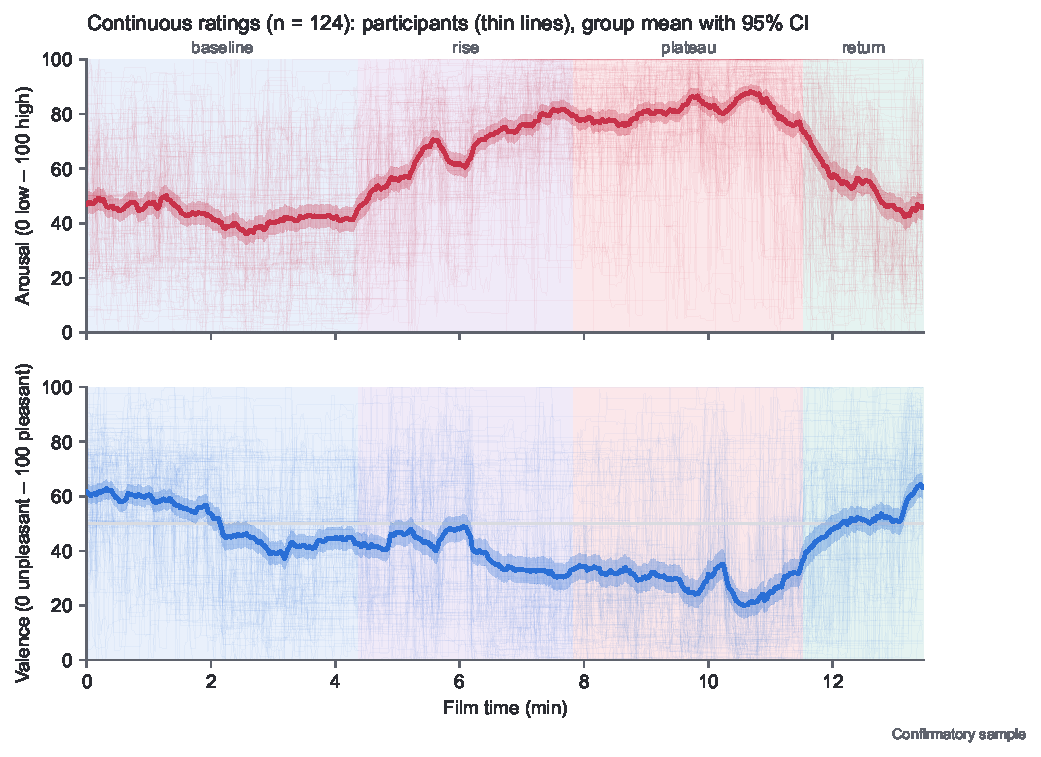
\includegraphics[width=\textwidth]{fig1_time_course.pdf}
\figurenote{Thin lines show individual participants; the thick line is the group mean with its 95\% confidence
interval ($N$~=~\val{n_primary}). Shading marks the four preregistered segments (baseline, rise, plateau, return).}
\end{figure}

\subsection{Confirmatory Analyses}

Table~\ref{tab:confirmatory} lists all preregistered tests for the primary sample. Ten of the 12 directional
predictions were supported, as were both replication criteria.

\begin{table}[tbp]
\caption{Preregistered Confirmatory Tests, Primary Sample}
\label{tab:confirmatory}
\begin{threeparttable}
\footnotesize\linespread{1}\selectfont\setlength{\tabcolsep}{3.5pt}
\begin{tabular}{@{}l>{\raggedright\arraybackslash}p{3.0cm}cllll@{}}
\toprule
Hypothesis & Prediction & Test statistic & Effect size [95\% CI] & $p$ & $p_\mathrm{Holm}$ & Supported \\
\midrule
H1 & STICSA somatic: post $>$ pre & $t$(123) = 11.46 & $d_z$ = 1.03 [0.81, 1.25] & $<$ .001 & -- & Yes \\
\addlinespace
H2a & Arousal: rise $>$ baseline & $t$(123) = 14.67 & $d_z$ = 1.32 [1.07, 1.56] & $<$ .001 & $<$ .001 & Yes \\
H2b & Arousal: plateau $>$ baseline & $t$(123) = 19.77 & $d_z$ = 1.78 [1.49, 2.06] & $<$ .001 & $<$ .001 & Yes \\
H2c & Arousal: return $<$ plateau & $t$(123) = $-$14.70 & $d_z$ = $-$1.32 [$-$1.56, $-$1.08] & $<$ .001 & $<$ .001 & Yes \\
H2d & Valence: plateau $<$ baseline & $t$(123) = $-$9.85 & $d_z$ = $-$0.88 [$-$1.09, $-$0.68] & $<$ .001 & $<$ .001 & Yes \\
\addlinespace
H3 arousal & Arousal curve replicates & -- & $r$ = .993 [.990, .996] & -- & -- & Yes \\
H3 valence & Valence curve replicates & -- & $r$ = .937 [.893, .966] & -- & -- & Yes \\
\addlinespace
H4a & Fear of heights, plateau arousal (+) & -- & $\rho$ = .08 [$-$.09, .26] & .355 & .355 & No \\
H4b & Fear of heights, plateau valence ($-$) & -- & $\rho$ = $-$.32 [$-$.46, $-$.16] & $<$ .001 & .001 & Yes \\
H4c & Fear of heights, STICSA change (+) & -- & $\rho$ = .18 [.00, .35] & .049 & .098 & No \\
\addlinespace
H5a & STICSA change, whole-film arousal (+) & -- & $\rho$ = .24 [.05, .41] & .008 & .008 & Yes \\
H5b & STICSA change, whole-film valence ($-$) & -- & $\rho$ = $-$.38 [$-$.51, $-$.23] & $<$ .001 & $<$ .001 & Yes \\
\addlinespace
H6a & Overall anxiety, STICSA change (+) & -- & $\rho$ = .56 [.44, .67] & $<$ .001 & $<$ .001 & Yes \\
H6b & Overall anxiety, plateau arousal (+) & -- & $\rho$ = .34 [.15, .50] & $<$ .001 & $<$ .001 & Yes \\
\bottomrule
\end{tabular}
\vspace{4pt}
\begin{tablenotes}[para,flushleft]
{\small\textit{Note.} $N$ = 124. H1 and H2: paired $t$ tests with $d_z$ and exact 95\% CIs (noncentral $t$). H3: Pearson $r$ between the confirmatory and exploratory group-mean series (808 one-second values), 95\% CI from a circular block bootstrap (30-s blocks, 5,000 resamples); supported if the lower bound exceeds .50. H4--H6: Spearman $\rho$ with percentile bootstrap 95\% CIs (5,000 resamples). Holm correction within H2 (four tests), H4 (three), H5 (two) and H6 (two); H1 is a single test. All tests two-sided; a directional hypothesis counts as supported only if significant in the predicted direction.}
\end{tablenotes}
\end{threeparttable}
\end{table}


\subsubsection{Somatic Anxiety Induction (H1)}

STICSA somatic scores were higher immediately after the film than immediately before it, by \val{H1:diff} points
on average (pre: $M$~=~\val{sticsa_pre_mean}, $SD$~=~\val{sticsa_pre_sd}; post: $M$~=~\val{sticsa_post_mean},
$SD$~=~\val{sticsa_post_sd}), \val{H1:report}. Scores rose for \val{n_increase} participants, did not change for
\val{n_nochange} and fell for \val{n_decrease}. Because many pre-film scores sat at the floor of the scale, we also
ran the registered Wilcoxon signed-rank test, which gave the same result (\val{H1:wilcoxon}). The increase was
spread across all eleven items rather than driven by one or two symptoms (Figure~\ref{fig:sticsa}); a racing heart
and muscle tension were the sensations most often endorsed after the film. H1 was supported.

\begin{figure}[tbp]
\caption{Somatic Anxiety Before and After the Film}
\label{fig:sticsa}
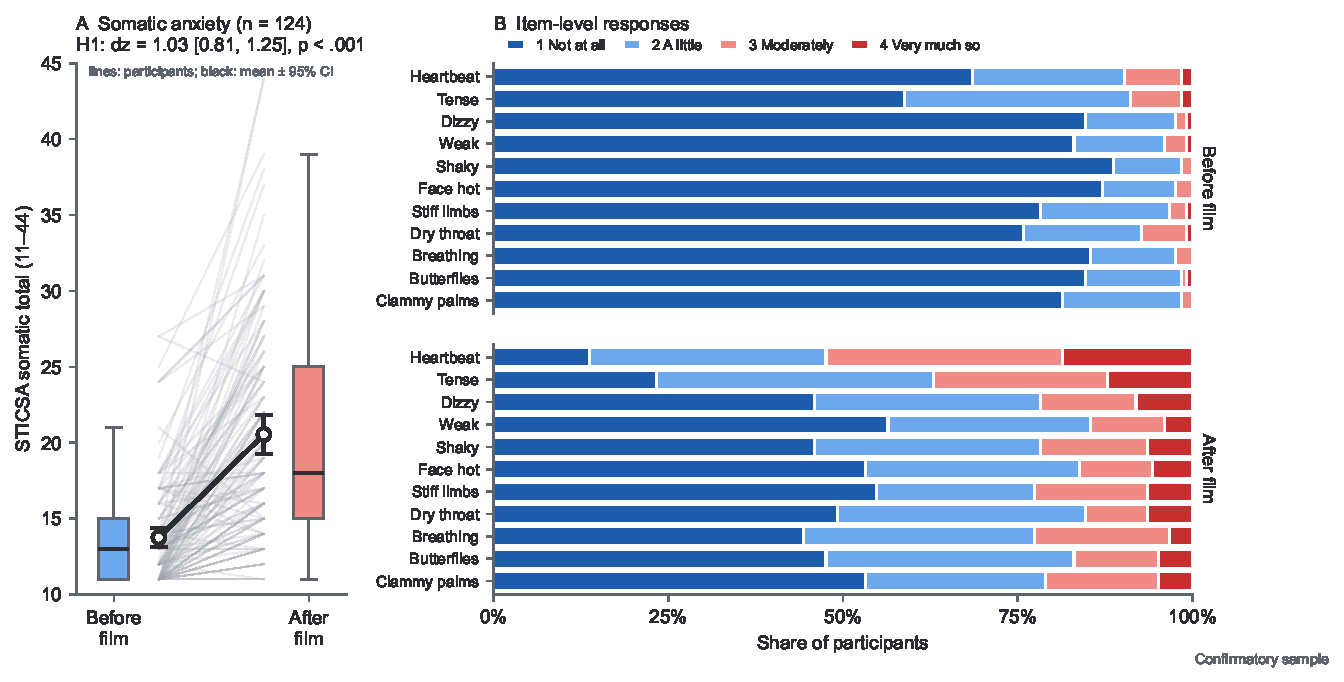
\includegraphics[width=\textwidth]{fig2_sticsa.pdf}
\figurenote{(A) STICSA somatic totals. Grey lines connect each participant's scores; boxes show medians and
interquartile ranges; the black line shows means with 95\% confidence intervals. (B) Share of participants giving
each answer to the eleven somatic items before (top) and after (bottom) the film.}
\end{figure}

\subsubsection{Affective Time Course (H2)}

All four segment contrasts went in the predicted direction and remained significant after Holm correction
(Figure~\ref{fig:segments}). Compared with the baseline, arousal was higher during the rise, by \val{H2a:diff}
points on the 0--100 scale, \val{H2a:report} (H2a), and higher still during the plateau, by \val{H2b:diff} points,
\val{H2b:report} (H2b). From the plateau to the return, arousal fell by \val{H2c:diffabs} points,
\val{H2c:report} (H2c). Valence was lower on the plateau than at baseline, by \val{H2d:diffabs} points,
\val{H2d:report} (H2d). The arousal effects were larger than the valence effect, partly because valence ratings
varied more between participants on the plateau ($SD$~=~\val{valence_plateau_sd}, against
\val{arousal_plateau_sd} for arousal).

\begin{figure}[tbp]
\caption{Mean Ratings in the Four Preregistered Segments}
\label{fig:segments}
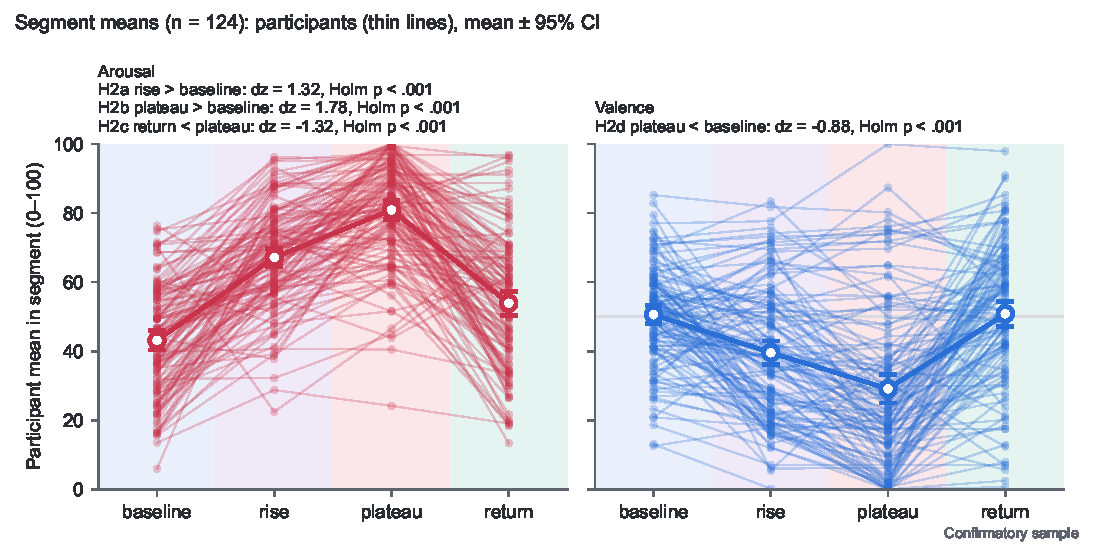
\includegraphics[width=\textwidth]{fig3_segment_means.pdf}
\figurenote{Each thin line is one participant's segment means; the thick line shows group means with 95\%
confidence intervals. Panel headings give the H2 contrasts with $d_z$ and Holm-adjusted $p$ values.}
\end{figure}

\subsubsection{Replication of the Group Time Course (H3)}

The group-mean time series of the confirmatory sample closely followed that of the independent exploratory sample
(Figure~\ref{fig:replication}). For arousal, \val{H3arousal:report}, and for valence, \val{H3valence:report}. In both
cases the lower bound of the confidence interval lay well above the preregistered criterion of .50, so H3 was
supported for both dimensions. The two arousal curves had almost the same shape but differed somewhat in level:
the confirmatory sample rated arousal a little higher during the baseline and the final minutes, and a little lower
on the plateau.

\begin{figure}[tbp]
\caption{Group-Mean Time Series in the Confirmatory and Exploratory Samples}
\label{fig:replication}
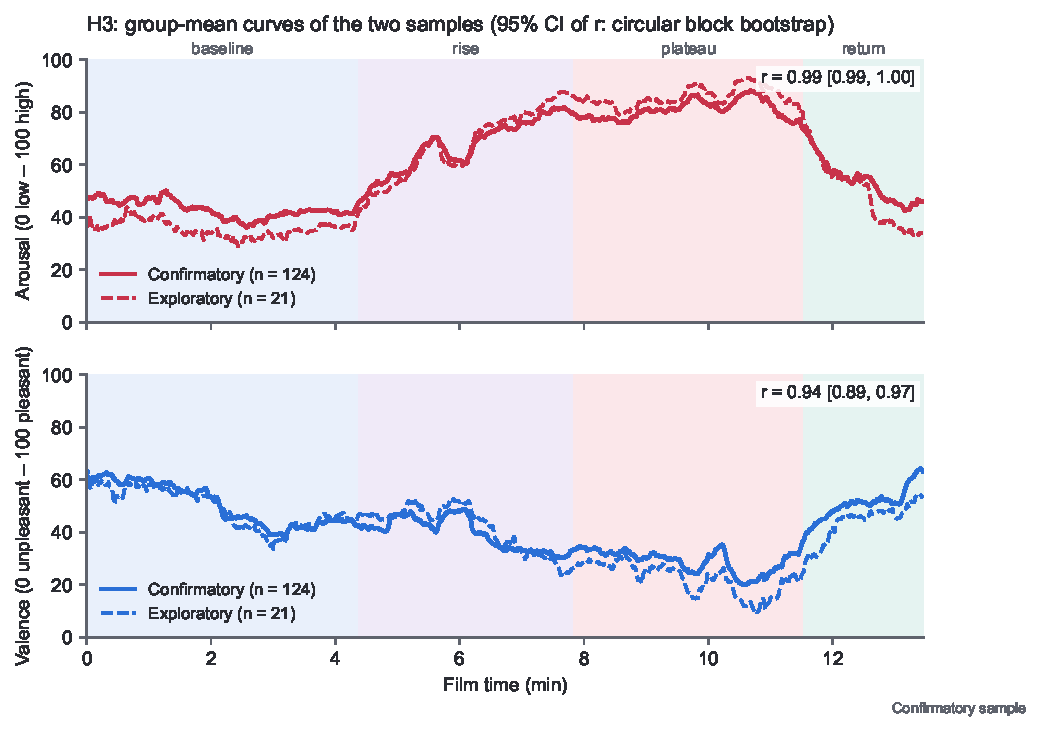
\includegraphics[width=\textwidth]{fig4_replication.pdf}
\figurenote{Solid lines: confirmatory sample ($n$~=~\val{n_primary}); dashed lines: exploratory sample
($n$~=~\val{n_exploratory}). Pearson $r$ is computed over the 808 one-second values; the 95\% confidence interval
comes from a circular block bootstrap with 30-s blocks.}
\end{figure}

\subsubsection{Individual Differences (H4--H6)}

Everyday fear of heights was related to how unpleasant the plateau felt, but not to how arousing it was or to the
change in somatic anxiety (Figure~\ref{fig:correlations}). Participants with a greater fear of heights rated
valence on the plateau as more negative, \val{H4b:report} (H4b). The predicted positive correlations with plateau
arousal, \val{H4a:report} (H4a), and with the STICSA change, \val{H4c:report} (H4c), were not supported; the latter
was significant only before correction.

The change in somatic anxiety was related to the continuous ratings as predicted. Participants whose STICSA scores
rose more gave higher arousal ratings over the whole film, \val{H5a:report} (H5a), and lower valence ratings,
\val{H5b:report} (H5b).

Overall anxiety reported after the film converged with both other measures. It correlated with the STICSA change,
\val{H6a:report} (H6a), and with plateau arousal, \val{H6b:report} (H6b). Both H5 and H6 were supported.

\begin{figure}[tbp]
\caption{Individual Differences Tested in H4--H6}
\label{fig:correlations}
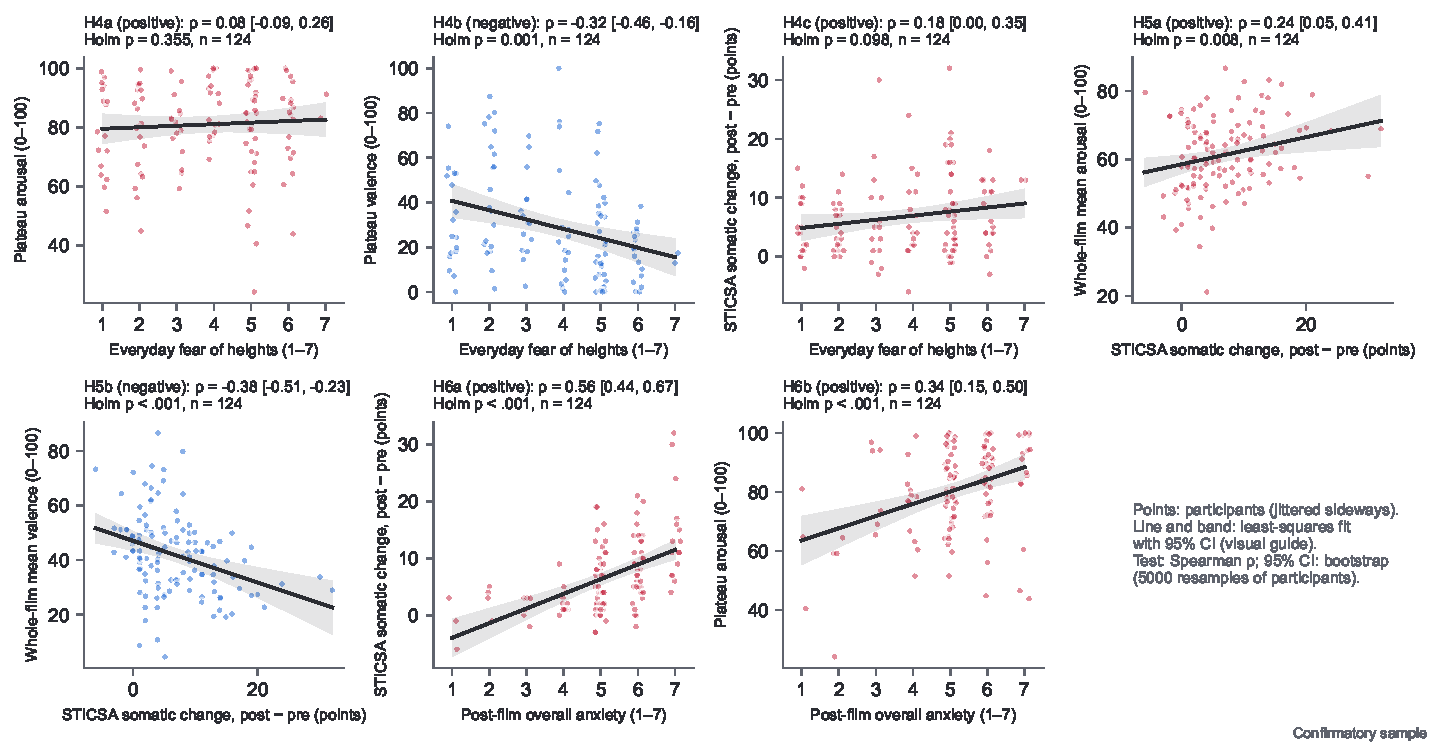
\includegraphics[width=\textwidth]{fig5_correlations.pdf}
\figurenote{Points are participants (shifted sideways slightly so that equal scores remain visible). The black line
and grey band show a least-squares fit with its 95\% confidence interval, drawn as a visual guide; the tests are
Spearman correlations. Panel headings give Spearman $\rho$ with bootstrap 95\% confidence intervals and
Holm-adjusted $p$ values.}
\end{figure}

\subsubsection{Sensitivity Analyses}

Repeating every test in the two sensitivity samples did not change any conclusion (Table~\ref{tab:sensitivity}).
The same ten directional predictions and both replication criteria were supported in each sample, and H4a and
H4c were not supported in either. Effect sizes stayed close to those in the primary sample; the segment contrasts
for arousal were somewhat larger when sparse and less engaged raters were removed.

\begin{table}[tbp]
\caption{Preregistered Tests Repeated in the Sensitivity Samples}
\label{tab:sensitivity}
\begin{threeparttable}
\footnotesize\linespread{1}\selectfont\setlength{\tabcolsep}{3.5pt}
\begin{tabular}{@{}llccc@{}}
\toprule
Hypothesis & Effect & Primary ($n$ = 124) & Stricter engagement ($n$ = 96) & Rejection set removed ($n$ = 120) \\
\midrule
H1 & $d_z$ & 1.03 ($p$ < .001) & 1.09 ($p$ < .001) & 1.02 ($p$ < .001) \\
H2a & $d_z$ & 1.32 ($p_\mathrm{Holm}$ < .001) & 1.51 ($p_\mathrm{Holm}$ < .001) & 1.43 ($p_\mathrm{Holm}$ < .001) \\
H2b & $d_z$ & 1.78 ($p_\mathrm{Holm}$ < .001) & 1.94 ($p_\mathrm{Holm}$ < .001) & 1.85 ($p_\mathrm{Holm}$ < .001) \\
H2c & $d_z$ & $-$1.32 ($p_\mathrm{Holm}$ < .001) & $-$1.65 ($p_\mathrm{Holm}$ < .001) & $-$1.39 ($p_\mathrm{Holm}$ < .001) \\
H2d & $d_z$ & $-$0.88 ($p_\mathrm{Holm}$ < .001) & $-$0.88 ($p_\mathrm{Holm}$ < .001) & $-$0.87 ($p_\mathrm{Holm}$ < .001) \\
H3 arousal & $r$ & .993 (lower .990) & .990 (lower .984) & .993 (lower .989) \\
H3 valence & $r$ & .937 (lower .893) & .925 (lower .869) & .927 (lower .876) \\
H4a & $\rho$ & .08 ($p_\mathrm{Holm}$ = .355)$^\dagger$ & .03 ($p_\mathrm{Holm}$ = .775)$^\dagger$ & .08 ($p_\mathrm{Holm}$ = .380)$^\dagger$ \\
H4b & $\rho$ & $-$.32 ($p_\mathrm{Holm}$ = .001) & $-$.30 ($p_\mathrm{Holm}$ = .010) & $-$.32 ($p_\mathrm{Holm}$ = .001) \\
H4c & $\rho$ & .18 ($p_\mathrm{Holm}$ = .098)$^\dagger$ & .21 ($p_\mathrm{Holm}$ = .088)$^\dagger$ & .17 ($p_\mathrm{Holm}$ = .142)$^\dagger$ \\
H5a & $\rho$ & .24 ($p_\mathrm{Holm}$ = .008) & .24 ($p_\mathrm{Holm}$ = .018) & .24 ($p_\mathrm{Holm}$ = .008) \\
H5b & $\rho$ & $-$.38 ($p_\mathrm{Holm}$ < .001) & $-$.32 ($p_\mathrm{Holm}$ = .003) & $-$.39 ($p_\mathrm{Holm}$ < .001) \\
H6a & $\rho$ & .56 ($p_\mathrm{Holm}$ < .001) & .49 ($p_\mathrm{Holm}$ < .001) & .56 ($p_\mathrm{Holm}$ < .001) \\
H6b & $\rho$ & .34 ($p_\mathrm{Holm}$ < .001) & .29 ($p_\mathrm{Holm}$ = .004) & .36 ($p_\mathrm{Holm}$ < .001) \\
\bottomrule
\end{tabular}
\vspace{4pt}
\begin{tablenotes}[para,flushleft]
{\small\textit{Note.} Cells show the effect size and, in parentheses, the Holm-adjusted $p$ value (H1: unadjusted, single test) or, for H3, the lower bound of the 95\% CI of $r$. $^\dagger$Hypothesis not supported under the registered criteria. Stricter engagement: sparse raters (fewer than one rating bout per minute or more than 180 s without input), participants who failed one attention check and participants who reported not watching attentively removed. Rejection set removed: participants whose Prolific submissions were rejected for behaviour on the free-text page removed, although they pass the registered exclusion rules.}
\end{tablenotes}
\end{threeparttable}
\end{table}


\subsection{Preregistered Descriptive Analyses}

The group-mean time series were highly reliable. Split-half reliability (1,000 random splits, Spearman--Brown
corrected) was \val{rel:arousal} for arousal and \val{rel:valence} for valence.

Re-estimating the segment edges in the confirmatory sample with the same piecewise-linear method placed the first
edge at \val{edge1:est}~s (participant-bootstrap 95\% interval \val{edge1:ci}), identical to the registered value of
\val{edge1:reg}~s, and the second at \val{edge2:est}~s \val{edge2:ci}, against \val{edge2:reg}~s registered. The third
edge, the start of the return, came out at \val{edge3:est}~s \val{edge3:ci}, about half a minute earlier than the
registered \val{edge3:reg}~s, which lies just outside the interval. The first two intervals are wide, reflecting a
gradual rise rather than a sharp change. As preregistered, all tests used the fixed edges.

\subsection{Exploratory Analysis: The Affect Grid by Film Phase}

The following analysis was not preregistered as a test and is purely descriptive. Figure~\ref{fig:grid} shows where
on the valence--arousal grid participants spent their time in each segment. At baseline, ratings were spread around
the centre of the grid with a slight lean towards low arousal. During the rise they moved upwards and to the left.
On the plateau most participants converged on the high-arousal, unpleasant corner, which was by far the most
occupied region of the grid at any point in the film. During the return they dispersed again around the centre,
with roughly as many participants on the pleasant as on the unpleasant side.

\begin{figure}[tbp]
\caption{Occupancy of the Affect Grid in Each Film Segment (Exploratory)}
\label{fig:grid}
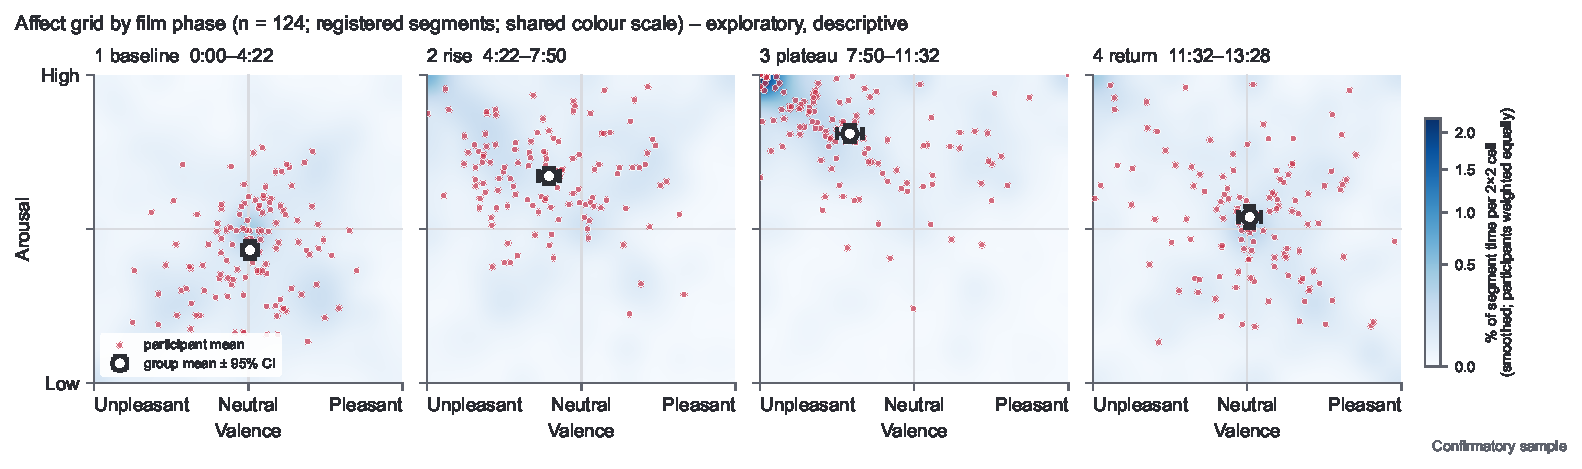
\includegraphics[width=\textwidth]{fig6_affect_grid_by_phase.pdf}
\figurenote{Blue shading shows the share of viewing time spent in each region of the grid (smoothed; each
participant weighted equally; same colour scale in all panels). Dots are participants' mean ratings in the segment;
the open circle is the group mean with 95\% confidence intervals.}
\end{figure}

\subsection{Exploratory Analysis: Age and Sex}

Age and sex were available for \val{n_demo} participants of the primary sample (\val{n_demo_female} female,
\val{n_demo_male} male). The film affected women and men, and younger and older participants, in much the same way
(Table~\ref{tab:agesex}).

The STICSA somatic score rose by \val{change_female_mean} points on average in women and \val{change_male_mean}
points in men. Adjusted for age, the difference (female minus male) was \val{agesex:change_sex}, and the change did not
depend on age (per 10 years, \val{agesex:change_age}; Figure~\ref{fig:agesex}A and B).

The time course of the ratings did not differ by sex or by age (Figures~\ref{fig:sexcourse} and \ref{fig:agesex}C
and D). For arousal, neither the segment~$\times$~sex interaction (\val{agesex:arousal:sex_x_segment}) nor the
segment~$\times$~age interaction (\val{agesex:arousal:age_x_segment}) was significant, and the same was true for
valence (sex: \val{agesex:valence:sex_x_segment}; age: \val{agesex:valence:age_x_segment}). The clustered-regression
check agreed in every case (Table~\ref{tab:agesex}). Averaged over the film, women's valence ratings were somewhat
lower than men's, by \val{agesex:valence:female_minus_male}; the difference was largest during the rise
(\val{agesex:valence_rise_diff}), but neither was significant.

\begin{table}[tbp]
\caption{Exploratory Analyses of Age and Sex}
\label{tab:agesex}
\begin{threeparttable}
\footnotesize\linespread{1}\selectfont\setlength{\tabcolsep}{3.5pt}
\begin{tabular}{@{}llllll@{}}
\toprule
 & & \multicolumn{2}{l}{Main analysis} & \multicolumn{2}{l}{Clustered regression (check)} \\
\cmidrule(lr){3-4}\cmidrule(l){5-6}
Outcome & Effect & Test or estimate & $p$ & Test or estimate & $p$ \\
\midrule
STICSA change & Female $-$ male (points) & 0.66 [$-$1.77, 3.08] & .593 & -- & -- \\
 & Per 10 years of age (points) & 0.24 [$-$0.78, 1.25] & .645 & -- & -- \\
\addlinespace
Arousal & Segment $\times$ sex & $\chi^2$(3) = 0.28 & .964 & $F$(3, 120) = 0.08 & .969 \\
 & Segment $\times$ age & $\chi^2$(3) = 4.92 & .178 & $F$(3, 120) = 2.13 & .100 \\
 & Female $-$ male (film mean) & -- & -- & $-$0.50 [$-$4.47, 3.47] & .806 \\
 & Per 10 years (film mean) & -- & -- & $-$1.26 [$-$2.88, 0.37] & .129 \\
\addlinespace
Valence & Segment $\times$ sex & $\chi^2$(3) = 0.72 & .869 & $F$(3, 120) = 0.43 & .734 \\
 & Segment $\times$ age & $\chi^2$(3) = 1.84 & .607 & $F$(3, 120) = 0.50 & .682 \\
 & Female $-$ male (film mean) & -- & -- & $-$4.46 [$-$9.91, 0.99] & .108 \\
 & Per 10 years (film mean) & -- & -- & $-$0.74 [$-$2.96, 1.47] & .511 \\
\bottomrule
\end{tabular}
\vspace{4pt}
\begin{tablenotes}[para,flushleft]
{\small\textit{Note.} Exploratory analyses, not preregistered tests; $p$ values are uncorrected. $n$ = 121 participants of the primary sample with age and sex available. STICSA change: linear regression on sex and age. Segment means: random-intercept mixed model with segment (sum-coded) $\times$ (sex + age), interactions tested with likelihood-ratio tests (main analysis); the same model fitted by least squares with standard errors clustered by participant, interactions tested with Wald $F$ tests, is shown as a check, together with the main effects of sex and age averaged over the film. Age effects are per 10 years; sex effects are female minus male, in scale points.}
\end{tablenotes}
\end{threeparttable}
\end{table}


\begin{figure}[tbp]
\caption{Group-Mean Ratings by Sex (Exploratory)}
\label{fig:sexcourse}
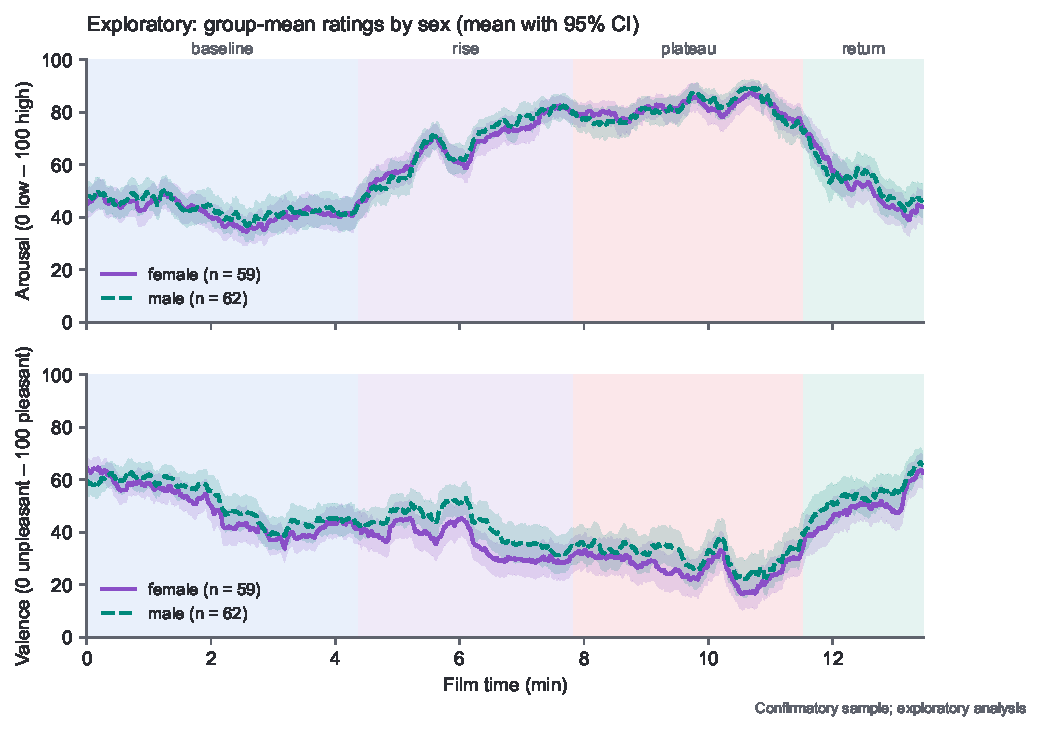
\includegraphics[width=\textwidth]{fig7_time_course_by_sex.pdf}
\figurenote{Group means with 95\% confidence intervals for female ($n$~=~\val{n_demo_female}, solid) and male
($n$~=~\val{n_demo_male}, dashed) participants. Shading marks the four preregistered segments.}
\end{figure}

\begin{figure}[tbp]
\caption{Somatic Anxiety Change and Segment Means by Sex and Age (Exploratory)}
\label{fig:agesex}
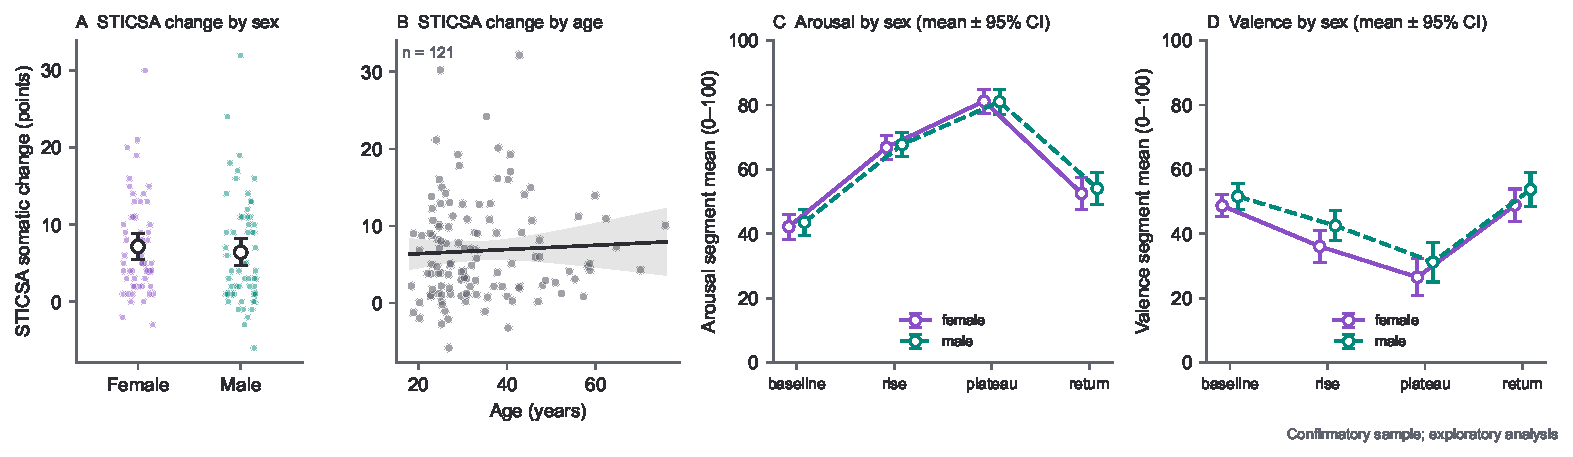
\includegraphics[width=\textwidth]{fig8_age_sex.pdf}
\figurenote{(A) STICSA somatic change by sex; points are participants, black markers means with 95\% confidence
intervals. (B) STICSA somatic change by age, with a least-squares line and 95\% confidence band as a visual guide;
points are jittered slightly because both variables take whole-number values. (C, D) Segment means of arousal and
valence by sex (means with 95\% confidence intervals). $n$~=~\val{n_demo}.}
\end{figure}

\subsection{Notes on the Preregistered Plan}

Five points should be read alongside the preregistration. First, the registration reported 123 usable confirmatory
participants at submission; one further participant completed the study after that count was made, had complete
data and passed all exclusion rules, and was included as registered ($N$~=~\val{n_primary}). Second, the fixed
segment edges were estimated on 22 exploratory participants under the quality-control rules in use at the time; under
the final registered rules, 21 of them are usable, and these 21 form the reference curve for H3. Third, one
participant's Prolific rejection was reversed for payment reasons after the registration; the participant remains in
the registered rejection set for the sensitivity analysis. Fourth, \enquote{reported not watching attentively} was
implemented as answering \enquote{No} to the attentiveness question; participants who answered \enquote{Mostly}
were retained. Fifth, in the exploratory age and sex analyses, the first confirmatory run reported the mixed models
as not converging. This was caused by the optimization algorithm, which failed on these data while three other
algorithms converged to the same solution; the code was corrected to try algorithms in turn, the model and decision
rule were left unchanged, and the analysis was rerun. The registration's example of mixed models over the 1-Hz series
was not implemented; the models use segment means.

\end{document}
